%%%%%%%%%%%%%%%%%%%%%%%%%%%%%%%%%%%%%%%%%%%%%%%%%%%
%% P3: Phenomenology of Particle Physics                         
%%
%% Author:  André Rubbia                   		 
%%
%% Figure 3.25 The velocity parameter $\beta=v/c$ as a function of momentum for pions, kaons, and protons.
%%
%% This work is licensed under the Creative Commons Attribution 4.0 International License. 
%% To view a copy of this license, visit http://creativecommons.org/licenses/by/4.0/ or 
%% send a letter to Creative Commons, PO Box 1866, Mountain View, CA 94042, USA.
%%
%%%%%%%%%%%%%%%%%%%%%%%%%%%%%%%%%%%%%%%%%%%%%%%%%%%

\documentclass[a4paper,10pt]{article}

\usepackage[T1]{fontenc}
\usepackage[utf8]{inputenc}
\usepackage{lmodern}
\usepackage[labelfont=bf]{caption}
\usepackage{upgreek}

\usepackage{tikz}
\usepackage{pgfplots}
\pgfplotsset{compat=1.17}
\usepgfplotslibrary{ternary}
\usepgfplotslibrary{fillbetween}
\usepgfplotslibrary{external}

\def\d{\mathrm{d}}

\usepackage{listings}

\begin{document}


%%%%%%%%%%%%%%%   FIGURE  %%%%%%%%%%%%%%%%%%%%%%%%%%%%%%
\begin{figure}[htb]
\begin{center}
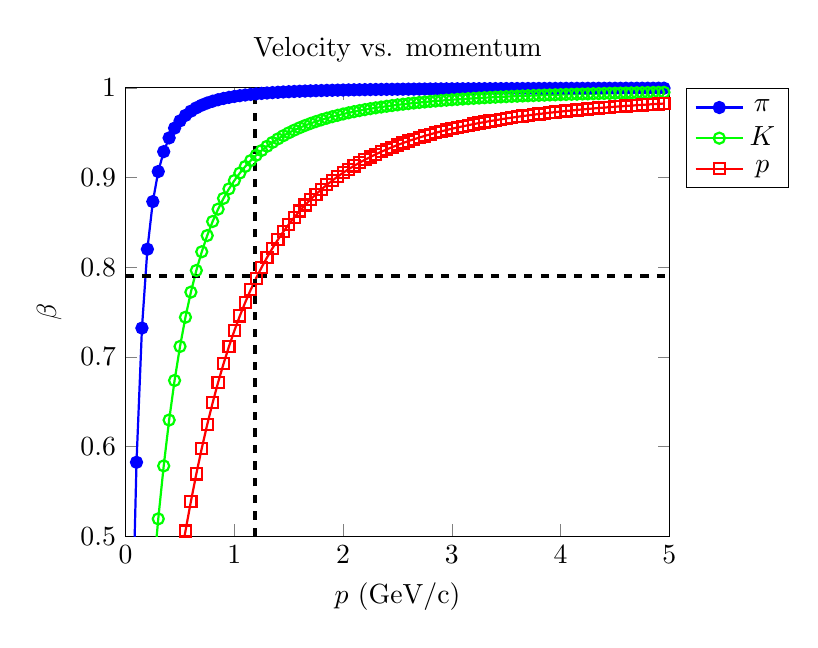
\begin{tikzpicture}[scale=1]
\begin{axis}[
    width=0.7\textwidth,
    height=0.6\textwidth,
    title={Velocity vs. momentum},
    xlabel={$p$ (GeV/c)},
    ylabel={$\beta$},
    xmin=0, xmax=5,
    ymin=0.5, ymax=1,
    legend pos=outer north east,
]
%% pion
\addplot[
    color=blue, thick, mark=*
    ]
    coordinates {
    (0,0)(0.05,0.337255)(0.1,0.582422)(0.15,0.732101)(0.2,0.820059)(0.25,0.873146)(0.3,0.906681)(0.35,0.92887)(0.4,0.944174)(0.45,0.955115)(0.5,0.963179)(0.55,0.969278)(0.6,0.973995)(0.65,0.977715)(0.7,0.980696)(0.75,0.983122)(0.8,0.98512)(0.85,0.986786)(0.9,0.988188)(0.95,0.989379)(1,0.9904)(1.05,0.991281)(1.1,0.992046)(1.15,0.992716)(1.2,0.993304)(1.25,0.993824)(1.3,0.994286)(1.35,0.994698)(1.4,0.995067)(1.45,0.995399)(1.5,0.995699)(1.55,0.99597)(1.6,0.996217)(1.65,0.996442)(1.7,0.996647)(1.75,0.996835)(1.8,0.997007)(1.85,0.997166)(1.9,0.997313)(1.95,0.997448)(2,0.997574)(2.05,0.99769)(2.1,0.997799)(2.15,0.9979)(2.2,0.997994)(2.25,0.998082)(2.3,0.998164)(2.35,0.998241)(2.4,0.998313)(2.45,0.998381)(2.5,0.998445)(2.55,0.998505)(2.6,0.998562)(2.65,0.998616)(2.7,0.998667)(2.75,0.998715)(2.8,0.99876)(2.85,0.998803)(2.9,0.998844)(2.95,0.998883)(3,0.99892)(3.05,0.998955)(3.1,0.998988)(3.15,0.99902)(3.2,0.99905)(3.25,0.999079)(3.3,0.999107)(3.35,0.999133)(3.4,0.999159)(3.45,0.999183)(3.5,0.999206)(3.55,0.999228)(3.6,0.999249)(3.65,0.99927)(3.7,0.999289)(3.75,0.999308)(3.8,0.999326)(3.85,0.999344)(3.9,0.99936)(3.95,0.999376)(4,0.999392)(4.05,0.999407)(4.1,0.999421)(4.15,0.999435)(4.2,0.999448)(4.25,0.999461)(4.3,0.999474)(4.35,0.999486)(4.4,0.999497)(4.45,0.999509)(4.5,0.999519)(4.55,0.99953)(4.6,0.99954)(4.65,0.99955)(4.7,0.999559)(4.75,0.999569)(4.8,0.999578)(4.85,0.999586)(4.9,0.999595)(4.95,0.999603)
    };


%% kaon
\addplot[
    color=green, thick, mark=o
    ]
    coordinates {
    (0,0)(0.05,0.100765)(0.1,0.19853)(0.15,0.290719)(0.2,0.37548)(0.25,0.451778)(0.3,0.519316)(0.35,0.578361)(0.4,0.629537)(0.45,0.673658)(0.5,0.711592)(0.55,0.744184)(0.6,0.772208)(0.65,0.796353)(0.7,0.81721)(0.75,0.835286)(0.8,0.851007)(0.85,0.864732)(0.9,0.87676)(0.95,0.88734)(1,0.896684)(1.05,0.904965)(1.1,0.912332)(1.15,0.918908)(1.2,0.924798)(1.25,0.93009)(1.3,0.934861)(1.35,0.939173)(1.4,0.943083)(1.45,0.946638)(1.5,0.949878)(1.55,0.952838)(1.6,0.955549)(1.65,0.958037)(1.7,0.960327)(1.75,0.962437)(1.8,0.964386)(1.85,0.96619)(1.9,0.967863)(1.95,0.969416)(2,0.97086)(2.05,0.972207)(2.1,0.973463)(2.15,0.974637)(2.2,0.975735)(2.25,0.976765)(2.3,0.977731)(2.35,0.978639)(2.4,0.979493)(2.45,0.980297)(2.5,0.981055)(2.55,0.981771)(2.6,0.982447)(2.65,0.983086)(2.7,0.983692)(2.75,0.984266)(2.8,0.98481)(2.85,0.985327)(2.9,0.985818)(2.95,0.986285)(3,0.986729)(3.05,0.987152)(3.1,0.987556)(3.15,0.987941)(3.2,0.988308)(3.25,0.988659)(3.3,0.988994)(3.35,0.989315)(3.4,0.989622)(3.45,0.989917)(3.5,0.990198)(3.55,0.990469)(3.6,0.990728)(3.65,0.990977)(3.7,0.991216)(3.75,0.991446)(3.8,0.991666)(3.85,0.991879)(3.9,0.992083)(3.95,0.99228)(4,0.99247)(4.05,0.992653)(4.1,0.992829)(4.15,0.992999)(4.2,0.993163)(4.25,0.993321)(4.3,0.993474)(4.35,0.993622)(4.4,0.993764)(4.45,0.993903)(4.5,0.994036)(4.55,0.994165)(4.6,0.99429)(4.65,0.994411)(4.7,0.994529)(4.75,0.994642)(4.8,0.994753)(4.85,0.994859)(4.9,0.994963)(4.95,0.995063)
      };

%% proton
\addplot[
    color=red, thick, mark=square
    ]
    coordinates {
    (0,0)(0.05,0.0532141)(0.1,0.105979)(0.15,0.157864)(0.2,0.208475)(0.25,0.257465)(0.3,0.304549)(0.35,0.349502)(0.4,0.392166)(0.45,0.432442)(0.5,0.470287)(0.55,0.505706)(0.6,0.53874)(0.65,0.569464)(0.7,0.597974)(0.75,0.624382)(0.8,0.648811)(0.85,0.671386)(0.9,0.692236)(0.95,0.711486)(1,0.729257)(1.05,0.745666)(1.1,0.760822)(1.15,0.774828)(1.2,0.787779)(1.25,0.799763)(1.3,0.810862)(1.35,0.82115)(1.4,0.830696)(1.45,0.839561)(1.5,0.847803)(1.55,0.855473)(1.6,0.862618)(1.65,0.869282)(1.7,0.875504)(1.75,0.881319)(1.8,0.886759)(1.85,0.891854)(1.9,0.89663)(1.95,0.901113)(2,0.905325)(2.05,0.909285)(2.1,0.913013)(2.15,0.916526)(2.2,0.919838)(2.25,0.922965)(2.3,0.925919)(2.35,0.928712)(2.4,0.931356)(2.45,0.93386)(2.5,0.936234)(2.55,0.938487)(2.6,0.940625)(2.65,0.942658)(2.7,0.94459)(2.75,0.946429)(2.8,0.948181)(2.85,0.94985)(2.9,0.951441)(2.95,0.95296)(3,0.95441)(3.05,0.955796)(3.1,0.957121)(3.15,0.958388)(3.2,0.959601)(3.25,0.960763)(3.3,0.961876)(3.35,0.962944)(3.4,0.963968)(3.45,0.964951)(3.5,0.965895)(3.55,0.966802)(3.6,0.967674)(3.65,0.968512)(3.7,0.969319)(3.75,0.970096)(3.8,0.970844)(3.85,0.971564)(3.9,0.972259)(3.95,0.972929)(4,0.973575)(4.05,0.974198)(4.1,0.9748)(4.15,0.975382)(4.2,0.975944)(4.25,0.976487)(4.3,0.977012)(4.35,0.977519)(4.4,0.978011)(4.45,0.978486)(4.5,0.978947)(4.55,0.979393)(4.6,0.979825)(4.65,0.980244)(4.7,0.98065)(4.75,0.981044)(4.8,0.981426)(4.85,0.981796)(4.9,0.982156)(4.95,0.982506)
    };

\draw[dashed, very thick] (axis cs:1.19,0.5)-- (axis cs:1.19,1);
\draw[dashed, very thick] (axis cs:0,0.79)-- (axis cs:5,0.79);

        \legend{$\pi$,$K$,$p$}
\end{axis}
\end{tikzpicture}
\caption{The velocity parameter $\beta=v/c$ as a function of momentum for pions,
kaons, and protons. The dashed lines correspond to the experimental setup described
in Section~15.9 of the book.}
\end{center}
\end{figure}
%%%%%%%%%%%%%%%   END FIGURE  %%%%%%%%%%%%%%%%%%%%%%%%%%%%%%

%%%%%%%%%%%%%%%%%%%%%%%%%%%%%%%%%%%%%%%%%%%%%%%%%%%
%%%%%%%%%%%%%%%%%%%%%%%%%%%%%%%%%%%%%%%%%%%%%%%%%%%

The $\beta$ values were generated with the following ROOT C++ macro:
\begin{lstlisting}[language=C++]
void plot(Double_t m) {
  for(int ip=0;ip<100;ip++) {
    Double_t pgev = ip/100.0*5;
    Double_t e=sqrt(pgev*pgev+m*m);
    Double_t beta = pgev/e;
    printf("(%g,%g)", pgev,beta);
  }
  printf("\n");
};

void betavsp()
{
  printf("---- pion ----\n");
  Double_t m=0.13957;   // rest mass in GeV
  plot(m);

  printf("---- proton ----\n");
  m=0.93827;
  plot(m);

  printf("---- kaon ----\n");
  m=0.493677;
  plot(m);
};
\end{lstlisting}
%%%%%%%%%%%%%%%%%%%%%%%%%%%%%%%%%%%%%%%%%%%%%%%%%%%
%%%%%%%%%%%%%%%%%%%%%%%%%%%%%%%%%%%%%%%%%%%%%%%%%%%
\end{document}
